% Created 2011-12-09 Fri 02:05
\documentclass[bigger, english, 10pt, presentation]{beamer}
\usepackage[utf8]{inputenc}
\usepackage[T1]{fontenc}
\usepackage{fixltx2e}
\usepackage{graphicx}
\usepackage{longtable}
\usepackage{float}
\usepackage{wrapfig}
\usepackage{soul}
\usepackage{textcomp}
\usepackage{marvosym}
\usepackage{wasysym}
\usepackage{latexsym}
\usepackage{amssymb}
\usepackage{hyperref}
\tolerance=1000
\usepackage{loochao}
\providecommand{\alert}[1]{\textbf{#1}}

\title{Group Meeting}
\author{Chao LU\thanks{chaol@princeton.edu}}
\date{2011-12-09 Fri}

\begin{document}

\maketitle

\begin{frame}
\frametitle{Outline}
\setcounter{tocdepth}{3}
\tableofcontents
\end{frame}



\section{Microscopy}
\label{sec-1}
\subsection{Microscopy}
\label{sec-1-1}
\begin{frame}
\frametitle{Film uniformity}
\label{sec-1-1-1}
\begin{columns}
\begin{column}{0.5\textwidth}
%% A block
\label{sec-1-1-1-1}

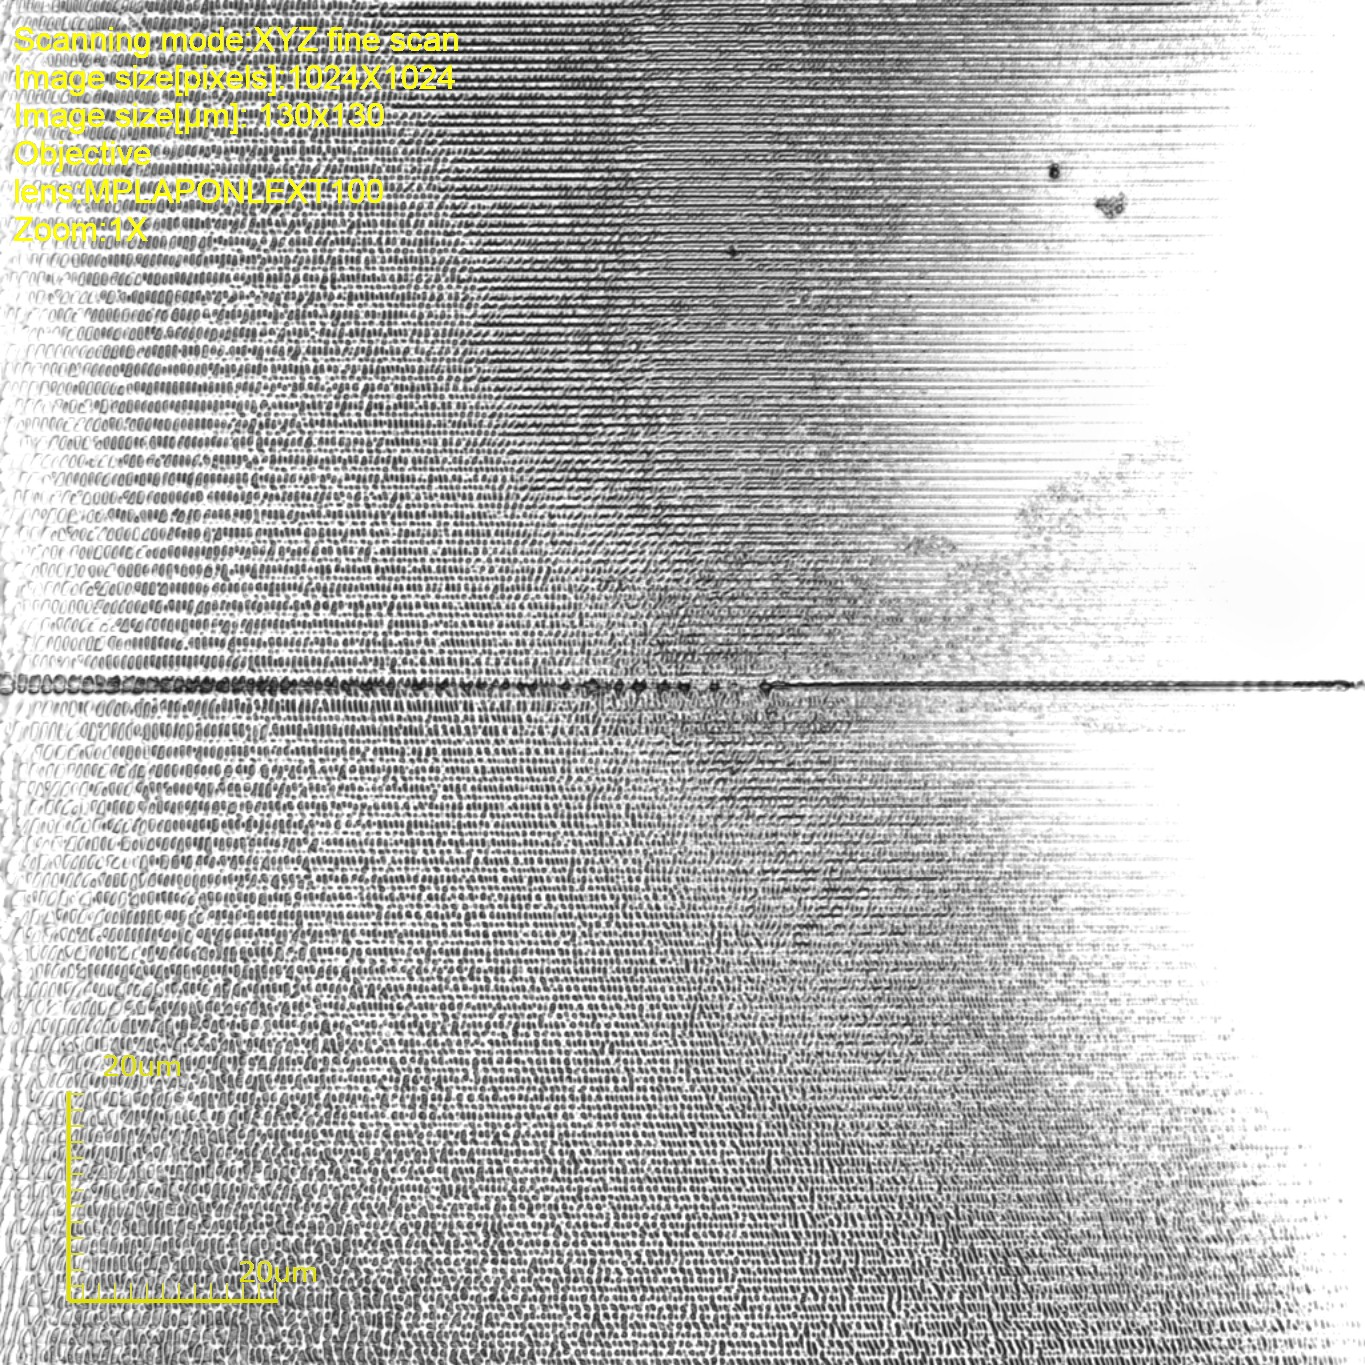
\includegraphics[width=.9\linewidth]{./figures/111208_As2S3_AsDep_UniformSite_100x_2D.jpg}
\end{column}
\begin{column}{0.6\textwidth}
\begin{example}[A screenshot]
\label{sec-1-1-1-2}

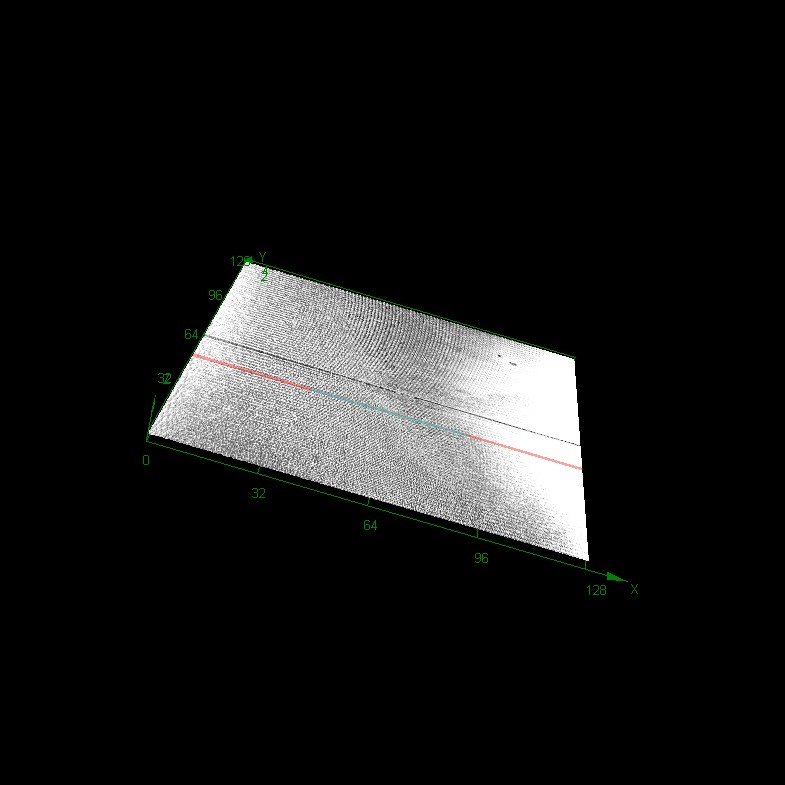
\includegraphics[width=.9\linewidth]{./figures/111208_As2S3_AsDep_UniformSite_100x_3D.jpg}
\end{example}
\end{column}
\end{columns}
\end{frame}
\begin{frame}
\frametitle{Short-range order}
\label{sec-1-1-2}

\begin{itemize}
\item medium-range order.
\end{itemize}
\end{frame}
\begin{frame}
\frametitle{Light induced phenomena}
\label{sec-1-1-3}
\end{frame}
\begin{frame}
\frametitle{Application}
\label{sec-1-1-4}
\end{frame}
\subsection{State of Art}
\label{sec-1-2}
\begin{frame}
\frametitle{The problem we're facing}
\label{sec-1-2-1}
\end{frame}
\begin{frame}
\frametitle{What others do about it}
\label{sec-1-2-2}
\end{frame}
\begin{frame}
\frametitle{What's the solution from our group}
\label{sec-1-2-3}
\end{frame}
\begin{frame}
\frametitle{Spin coating difference}
\label{sec-1-2-4}
\end{frame}
\section{Preliminary Results}
\label{sec-2}
\subsection{Theoretical (Volume expansion)}
\label{sec-2-1}
\begin{frame}
\frametitle{Dipole interaction mode}
\label{sec-2-1-1}
\end{frame}
\subsection{Experimental (Change of index of refraction)}
\label{sec-2-2}
\begin{frame}
\frametitle{Setup of the laser}
\label{sec-2-2-1}
\end{frame}
\begin{frame}
\frametitle{SEM image of As$_2$ S$_3$}
\label{sec-2-2-2}
\begin{theorem}[Org mode increases productivity]
\label{sec-2-2-2-1}

\begin{itemize}
\item org mode means not having to remember \LaTeX commands.
\item it is based on ascii text which is inherently portable.
\item Emacs!
\end{itemize}
\end{theorem}
\end{frame}
\begin{frame}
\frametitle{Volume gratings}
\label{sec-3-1}
\end{frame}
\begin{frame}
\frametitle{Hologram}
\label{sec-3-2}
\end{frame}
\begin{frame}
\frametitle{Creating structure by light}
\label{sec-3-3}
\end{frame}
\begin{frame}
\frametitle{Confirming defeats}
\label{sec-3-4}
\end{frame}
\begin{frame}
\frametitle{Craig}
\label{sec-4-1}

\begin{itemize}
\item Here's the problem we're dealing with.
\item Here how others
\end{itemize}
\end{frame}
\section{Future Challenges}
\label{sec-3}
\section{Backup slides}
\label{sec-4}

\end{document}